% Section content template for individual Educative lessons
% This file contains the actual content for a specific section
% Generated from Educative API section content

% Section: Design of a Distributed Task Scheduler
% Section ID: 4969977353863168
% Section Slug: design-of-a-distributed-task-scheduler
% Generated: 2025-12-07T22:09:18.743686

Let's identify the components used in this design:

\subsection{Components}\label{5pkQbVHELCXbPGYGYqPzh}
\\
We can consider scheduling at many levels. We could be asked to design scheduling that is done internally by an organization to run tasks on their own cluster of machines. There , they have to find ample resources and need to decide which task to run first.
\\
On the other hand, we could also be asked to design scheduling that a cloud provider uses to schedule tasks coming from multiple clients. Cloud providers need to decide which task to run first and which clients to handle first to provide appropriate isolation between different tenants.
\\
So, in general, the big components of our system are:

\begin{itemize}
\item
\protect\phantomsection\label{ASsfSPerbQwel06kWWLJM}
\textbf{Clients:} They initiate the task execution.
\item
\protect\phantomsection\label{_lGuoxAn-M7TN1cEY1xsx}
\textbf{Resources:} The task is executed on these components.
\item
\protect\phantomsection\label{ndLEBNKeuMXXu6yPFdbwS}
\textbf{Scheduler:} A scheduler performs processes between clients and resources and decides which task should get resources first.
\end{itemize}

\begin{figure}[htbp]
 \centering
 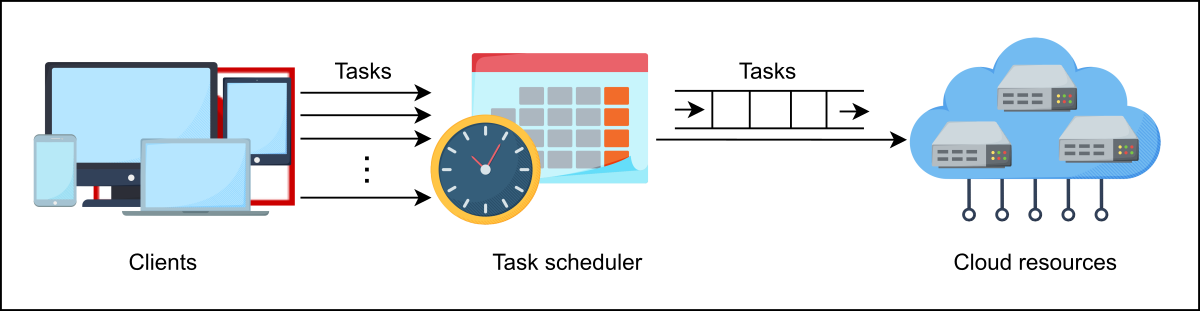
\includegraphics[width=0.5\textwidth]{Images/chapter_23/section_4969977353863168/5650193313038336.png}
 \caption{Scheduler putting tasks into a queue for resource allocation}
\end{figure}

As shown in the above illustration, it is necessary to put the incoming tasks into a \textbf{queue}. It is because of the following reasons:

\begin{itemize}
\item
\protect\phantomsection\label{xZib4nzJ2TYCPjisYlvbp}
We might not have sufficient resources available right now.
\item
\protect\phantomsection\label{a06ZRykVgJ_pialDGDxhj}
There is task dependency, and some tasks need to wait for others.
\item
\protect\phantomsection\label{SXhQSFPenJHlLtg23uF-3}
We need to decouple the clients from the task execution so that they can hand off work to our system. Our system then queues it for execution.
\end{itemize}
\\
Let's design a task scheduling system that should be able to schedule any task. Often , many tasks are relatively short-lived---from seconds to minutes. For long-running tasks, we might need the ability of periodic checksumming and restoration at the application level to recover from possible failures.
\\
Let's assume that some single server in our fleet can meet the computational needs of each task. For tasks that need many servers, either the application would need to break them down into smaller tasks for our system or employ long-term resource acquisition from the cluster manager.

\subsection{Design}\label{hr5xAwBErfwFq6URFVM4V}
\\
When a task comes for scheduling, it should contain the following information with it:

\begin{itemize}
\item
\protect\phantomsection\label{EEdrpsfrjQPBESrmarRIK}
\textbf{Resource requirements:} The requirements include how many CPU cores it needs, how much RAM is required to execute this task, how much disk space is required, what should the disk access rate be (input/output rate per second, or IOPS), and how many TCP ports the task needs for the execution, and so on. But, it is difficult for the clients to quantify these requirements. To remedy this situation, we have different tiers of resources like basic, regular, and premium. The client can specify the requirement in terms of these tiers.
\item
\protect\phantomsection\label{8BRUNEB0gck6ail8GjobA}
\textbf{Dependency:} Broadly, tasks can be of two types: dependent and independent.

\begin{itemize}
\item
\textbf{Dependent tasks} require executing one or more additional tasks for their complete execution. These tasks must run in a sequence. For a dependent task, the client should provide a list of the tasks on which a given task is dependent.
\item
\textbf{Independent task} s don't depend on the execution of any other task. Independent tasks can run in parallel. We should know whether a task is dependent or independent. The dependency information helps to execute both dependent tasks in order and independent tasks in parallel for efficient utilization of resources.
\end{itemize}
\end{itemize}
\\
The design of the task scheduler is shown in the following illustration:

\begin{figure}[htbp]
 \centering
 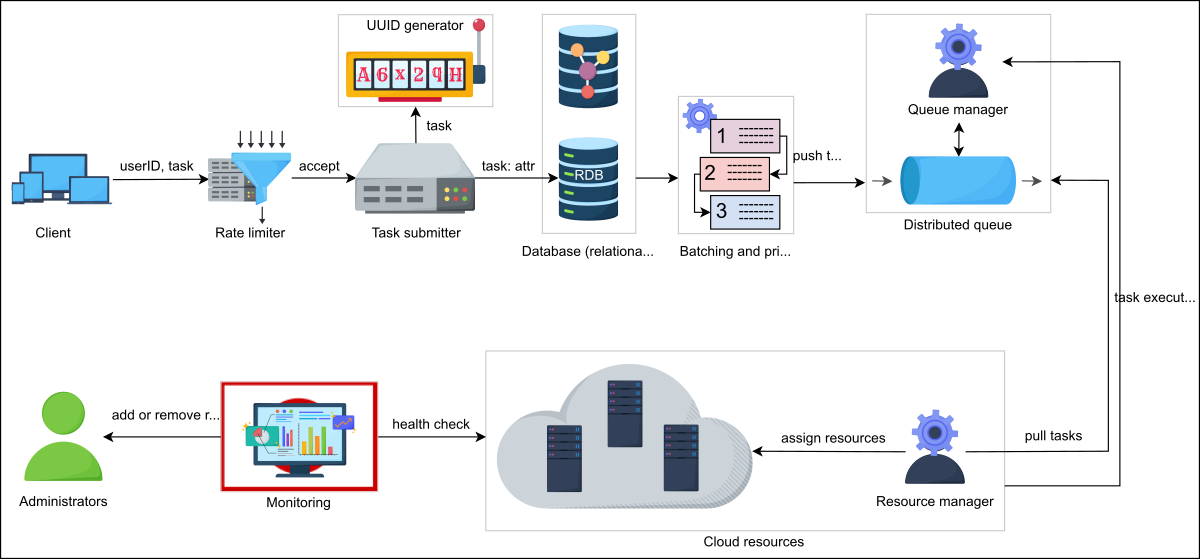
\includegraphics[width=0.5\textwidth]{Images/chapter_23/section_4969977353863168/6376229546885120.png}
 \caption{The design of task scheduler}
\end{figure}

\begin{itemize}
\item
\protect\phantomsection\label{vZoy7Xk0kYWalw8Jan4bU}
\textbf{Clients}: The clients of the cloud providers are individuals or organizations from small to large businesses who want to execute their tasks.
\item
\protect\phantomsection\label{2e-X1FLZmNZBmzkLhQ9f-}
\textbf{Rate limiter}: The resources available for a client depend on the cost they pay. It is important to limit the number of tasks for the reliability of our service. For instance, X number of tasks per hour are allowed to enter the system. Others will get a message like ``Limit exceeded'' instead of accepting the task and responding late. A rate limiter limits the number of tasks the client schedules based on its subscription. If the limit is exceeded, it returns an error message to the client that the rate limit has been exceeded.
\item
\protect\phantomsection\label{-yPu2vI-DQFlC9CqV7Bmv}
\textbf{Task submitter}: The task submitter admits the task if it successfully passes through the rate limiter. There isn't a single task submitter. Instead, we have a cluster of nodes that admit the increasing number of tasks.
\item
\protect\phantomsection\label{DhAa4YXH5qno0dLErmJZY}
\textbf{Unique ID generator}: It assigns unique IDs to the newly admitted tasks.
\item
\protect\phantomsection\label{44a0L8QmL3yFUS9hx43ry}
\textbf{Database}: All of the tasks taken by the task submitter are stored in a distributed database. For each task, we have some attributes, and all of the attributes except one are stored in the relational database.

\begin{itemize}
\item
\textbf{Relational database (RDB)}: A relational database stores task IDs, user IDs, required resources, execution caps, the total number of attempts made by the client, delay tolerance, and so on, as shown in the following table. We can find the details on the RDB \href{https://www.educative.io/courses/grokking-the-system-design-interview/types-of-databases}{here}.
\item
\textbf{Graph database (GDB)}: This is a non-relational database that uses the graph data structure to store data. We use it to build and store a directed acyclic graph (DAG) of dependent tasks, topologically sorted by the task submitter, so that we can schedule tasks according to that DAG. We can find more details of the graph DB \href{https://www.educative.io/courses/grokking-the-system-design-interview/types-of-databases}{here}.
\end{itemize}
\end{itemize}

\textbf{Database Schema}

\begin{table}[htbp]
\centering
\small
\adjustbox{max width=\textwidth}{
\begin{tabular}{|p{0.317\textwidth}|p{0.317\textwidth}|p{0.317\textwidth}|}
\hline
Column Name & Datatype & Description \\
\hline
\hline
TaskID & Integer & Uniquely identifies each task. \\
\hline
UserID & Integer & This is the ID of the task owner. \\
\hline
SchedulingType & VarChar & This can be either once, daily, weekly, monthly, or annually. \\
\hline
TotalAttempts & Integer & This is the maximum number of retries in case a task execution fails. \\
\hline
ResourceRequirements & VarChar & Clients have to specify the type of the offered resource categories, such as Basic, Regular, or Premium. The specified resource category is saved in the form of a string in the RDB. \\
\hline
ExecutionCap & Time & This is the maximum time allowed for the task execution. (This time starts when a resource is allocated to the task.) \\
\hline
Status & VarChar & This can be waiting, in progress, done, or failed. \\
\hline
DelayTolerance & Time & This indicates how much delay we can sustain before starting a task. \\
\hline
ScriptPath & VarChar & The path of the script that needs to be executed. The script is a file placed in a file system. The file should be made accessible so that it can be executed, just like how we mount Google Drive in the Google Colaboratory and then execute our code files there. \\
\hline
\end{tabular}
}
\caption{Database Schema}
\end{table}

\begin{quote}
\textbf{Note:} If we use geo-replicated data stores, we can run multiple instances of our task scheduling system in different data centers to achieve even larger scale and higher resource utilization.
\end{quote}
\begin{itemize}
\item
\protect\phantomsection\label{jNUn7E1B8ThgnrrMFT_rX}
\textbf{Batching and prioritization}: After we store the tasks in the RDB, the tasks are grouped into batches. Prioritization is based on the attributes of the tasks, such as delay tolerance or the tasks with short execution cap, and so on. The top K priority tasks are pushed into the distributed queue, where K limits the number of elements we can push into the queue. The value of K depends on many factors, such as currently available resources, the client or task priority, and subscription level.
\end{itemize}

\begin{quote}
\textbf{Quiz:}
\textbf{Question 1:} Why do we store tasks in a database? Why should we not push the tasks directly to the queue?
\textbf{Answer:} We do not push all tasks directly to the queue because not all of them are ready for immediate execution. Queues are designed for transient task handling and may have limited retention. If a task is scheduled for later or needs tracking and retries, we store it in a database to manage its lifecycle reliably. This approach also allows us to support different scheduling types, such as daily or monthly tasks, and gives the system flexibility to push tasks to the queue only when they are ready to be processed.
\end{quote}

\begin{itemize}
\item
\protect\phantomsection\label{5V1UmVfLbENKZpMwKF_jY}
\textbf{Distributed queue}: It consists of a queue and a queue manager. The queue manager adds, updates, or deletes tasks in the queue. It keeps track of the types of queues we use. It is also responsible for keeping the task in the queue until it executes successfully. In case a task execution fails, that task is made visible in the queue again. The queue manager knows which queue to run during the peak time and which queue to run during the off-peak time.
\item
\protect\phantomsection\label{VLiOOZeZbCcvgk4C5aB4j}
\textbf{Queue manager}: The queue manager deletes a task from the queue if it executes successfully. It also makes the task visible if its previous execution failed. It retries for the allowed number of attempts for a task in case of a failed execution.
\item
\protect\phantomsection\label{aZnctSbch00aKtFjsQrAg}
\textbf{Resource manager}: The resource manager knows which of the resources are free. It pulls the tasks from the distributed queue and assigns them resources. The resource manager keeps track of the execution of each task and sends back their statuses to the queue manager. If a task goes beyond its promised or required resource use, that task will be terminated, and the status is sent back to the task submitter, which will notify the client about the termination of the task through an error message.
\item
\protect\phantomsection\label{OOqDvXoTphBEYBbKPbTLY}
\textbf{Monitoring service}: It is responsible for checking the health of the resource manager and the resources. If some resource fails, it alerts the administrators to repair the resource or add new resources if required. If resources are not being used, it alerts the administrators to remove them or power them off. Here's \href{https://www.educative.io/courses/grokking-the-system-design-interview/system-design-distributed-monitoring}{a detailed discussion} on the design of monitoring services.
\end{itemize}

\subsection{Task submitter}\label{ERyJE69N_QDVujfKVr8mG}
\\
As we have seen above, every component we use in the design of the distributed task scheduler is distributed and therefore scalable and available. But , the task submitter could be a single point of failure. So, to handle this, we use a cluster of nodes. Each node must admit the tasks, send the tasks to a unique ID generator for ID assignment, and then store the task along with the task ID in the distributed database.
\\
There is a cluster manager to which each node sends a heartbeat that indicates the node is working correctly. Each node updates the cluster manager about the admitted tasks. The cluster manager maintains a list of tasks and the node ID that admitted that task. In case a node fails to execute a task, the cluster manager hands over that task to another node in the cluster. The cluster manager is itself replicated.
\\
Above, we designed a task scheduling system. We'll discuss the design considerations of our task scheduler in the next lesson.

% End of section content